\documentclass[12pt]{article}
\usepackage{fullpage,enumerate,amsmath,amssymb,graphicx, float}

\begin{document}
\begin{center}
{\Large CS224N Fall 2014 Programming Assignment 2}
\vspace{12pt}

SUNet ID: tzhang54, jiajihu

Name: Tong Zhang, Jiaji Hu
\vspace{12pt}
\end{center}

\section{Implementing a CKY Parser}
\subsection{Algorithm and Naive Implementation}
To implement the CKY Parser, we followed the pseudocode introduced in the videos. The main idea of the algorithm is that we build up the parse in a bottom-up manner. During the process, we store intermediate results to speed up the process.
As introduced in the videos, the time complexity of the CKY algorithm is $O(n^3)$.

We started with a naive implementation of the algorithm. Note that the key design choices in the implementation is what kind of data structure we choose to store the intermediate results. In particular, the two tables \texttt{score} and \texttt{back}.

From the very start, it was clear that we cannot use a 3-d array to store these tables, as the third dimension will be very large but sparse, due to the large number of distinct words in the treebank, and we will quickly run out of memory. Therefore, we chose to use a Hashmap data structure. We chose \texttt{HashMap<Triplet<Integer, Integer, String>, Double>} for \texttt{score}, and \texttt{HashMap<Triplet<Integer, Integer, String>, Triplet<Integer, String, String>>} for \texttt{back}. Also, to keep track of which tags had non-zero values in a block, we kept a \texttt{HashMap<Pair<Integer, Integer>, Set<String>>} called \texttt{tagDict} to get that set of tags.

Looking back, this setup was highly inefficient. Using the optimizations described below, we were able to dramatically improve our speed performance, resulting in a setup that could parse the test set in less than 3 minutes, averaging one parse per second, and handle sentences of length 20 in 2 seconds.
\subsection{Optimizations}
\subsubsection{Data Structures}
First, we came across the \texttt{CounterMap} data structure provided in the code library. We realized that it was quite convenient for our use case. Using a \texttt{CounterMap<Pair<Integer, Integer>, String>} for \texttt{score}, we were able to get rid of \texttt{tagDict}, since the information was already in the Map.

Next, we looked into using \texttt{IdentityHashMap} to further improve the speed of operations in \texttt{score}. Since a data structure that incorporated \texttt{IdentityHashMap} into \texttt{CounterMap} was not provided, we wrote our own \texttt{IndentityCounterMap}, which used an \texttt{IdentityHashMap} in the first step, which is \texttt{Pair<Integer, Integer>} to \texttt{String}. We didn't use it for the \texttt{String} to \texttt{Double} step because we figured that we would then need to get canonical representations for \texttt{String}s, which might be computationally heavy and also heavy on memory. In practice, doing that for Strings did negatively impact our performance.

For the \texttt{back} table, we also wanted to incorporate \texttt{IdentityHashMap}. We found out through trials that hashing and getting back \texttt{Triplet}s was slightly slower than our current solution (and also that there was a terrible bug in the skeleton code for \texttt{Triplet} that causes countless unnecessary hash collisions). We had the idea that since we were already using an \texttt{Interner<Pair<Integer, Integer>>} for \texttt{score}, we might as well utilize that also for \texttt{back}. Therefore, we came up with a similar data structure to \texttt{IdentityCounterMap}, and named it \texttt{IdentityTripletMap}. We implemented that class ourselves.

Using these data structures, we were able to dramatically improve our runtimes. In addition, we were able to shave a bit more off our runtime by doing code flow analysis.
\subsubsection{Code Analysis}
We carefully analyzed our code to see if we could save a bit of computation here and there. For example, by moving our interning towards the top of the loops, we could make sure that we didn't repeat that work.

Also, we looked at the \texttt{while(added)} loop given by the pseudocode in the videos. We see that the loop goes over all \texttt{A,B} in \texttt{nonterms} and \texttt{A->B in grammar}. We realized that on the second iteration of the loop, we really only need to look at the items newly added in the previous iteration. Therefore, if we just keep track, we can look at much fewer candidates for the unary rule in subsequent iterations. Implementing something to that effect actually sped up the runtime by around 10\%.

There were many similar tweaks to the code. By intuition and also trial and error, we worked out what data structures and what code flow allowed the parser to run faster.
\section{Adding Vertical Markovization}
\subsection{2nd Order Vertical Markovization Implementation}
We implemented vertical markovization to the unannotated tree in a recursive manner. Each node was passed in with the label of the parent node, and if the node is not a leaf, we update the new label to \texttt{childLabel \^\ parentLabel}. For \texttt{ROOT}, the parent label was an empty string.
\subsection{Effect Analysis}
As reported in the results section, adding 2nd order vertical markovization improved F1 score by \textbf{3\%} from 77.57 to 80.66. The number of exact match cases also increased by more than 10\%.

This improvement in results verified the points of integrating vertical markovization addressed in the \textit{Accurate Unlexicalized Parsing} paper. In the basic (1st order vertical) grammar, the cateogry symbols are too coarse to adequately render the expansions independent of the contexts. It is hard to differentiate various expansions from the same category without integrating ancestor labels.

\section{Results}
\subsection{Run Time}
\begin{center}
\begin{tabular}{|c|c|c|c|}
\hline
Algorithm & Total Runtime (s) & Avg. Runtime (s) & Length 20 (s)\\\hline
1st Order Vertical & 160.32 & 1.03 & 2.04 \\\hline
2nd Order Vertical & 253.54 & 1.64 & 3.50 \\\hline
3rd Order Vertical & 344.83  & 2.22 & 4.58 \\\hline
1st V + 1st H & 373.05 & 2.41 & 5.02 \\\hline
2nd V + 1st H & 352.20 & 2.27 & 4.68 \\\hline
\end{tabular}
\end{center}
Below is the graph for runtime versus sentence length for the basic parser with 1st order vertical markovization. Since the runtime should be $O(n^3)$, we fitted a third order polynomial curve to the data points. As shown below, the curve fits quite well.
\begin{figure}[H]
\centering
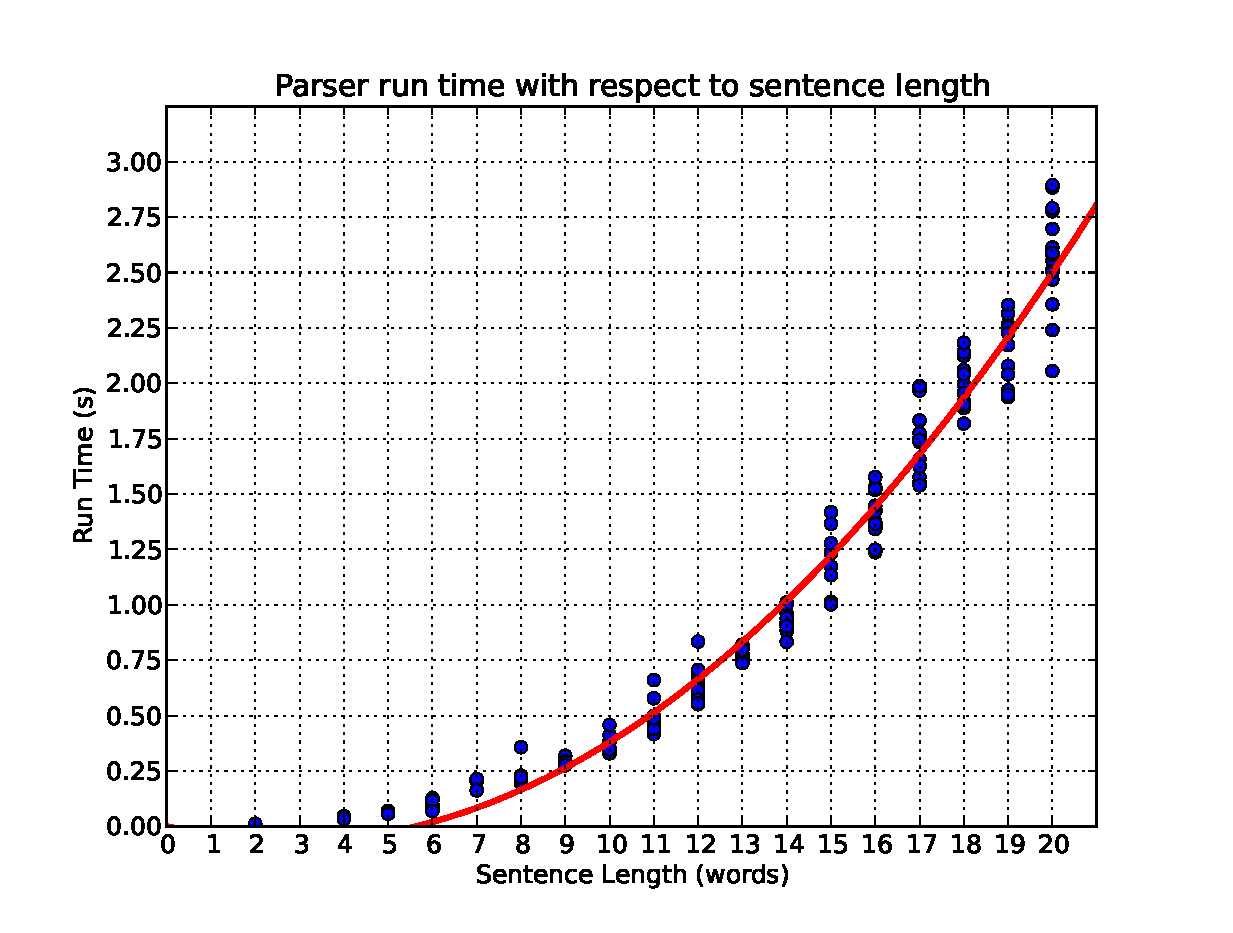
\includegraphics[width=0.5\linewidth]{./stats/runtime}
\end{figure}
\subsection{Parsing Score}
\begin{center}
\begin{tabular}{|c|c|c|c|c|}
\hline
Algorithm & Precision & Recall & $F_1$ & Exact Match \\\hline
1st Order Vertical & 80.76 & 74.63 & 77.57 & 20.65\\\hline
2nd Order Vertical & 83.64 & 79.73 & 81.64 & 31.61 \\\hline
3rd Order Vertical & 82.13 & 82.28 & 82.20 & 36.13 \\\hline
1st V + 1st H & 80.68 & 79.96 & 80.32 & 29.68 \\\hline
2nd V + 1st H & 84,94 & 85.60 & 85.27 & 34.19 \\\hline
\end{tabular}
\end{center}
\section{Extra Credit}
\subsection{Higher Order Vertical And Horizontal Markovization}
\subsubsection{3rd Order Vertical Markovization}
We implemented the 3rd order vertical markovization in a similar manner as the 2nd order one. At each recursive call, the grandparent node label was also passed in addtion to the parent node label. The label for the current node was updated to

\texttt{childLabel \^\ parentLabel \^\ grandparentLabel}. 
\subsubsection{Horizontal Markovization}
We also implemented 1st order and 2nd order horizontal markovizations. For n-th order horizontal markovization, we kept track of the previous n sibling labels as the context. Horizontal contexts are marked with \texttt{\^\ @}.
\subsubsection{Combination And Results}
We tried different combinations of vertical and horizontal markovizations and reported the results in the section above. 

\end{document}